\documentclass{beamer}
\usepackage[utf8]{inputenc}
\usetheme{Darmstadt}
\usepackage{hyperref}
\usepackage[T1]{fontenc}
\usepackage{latexsym,amsmath,xcolor,multicol,booktabs,calligra}
\usepackage{graphicx,pstricks,listings,stackengine}
\usepackage{lipsum}


\title{Simulateur d'écosystème}
\institute{Université de Caen Normandie}
\author{Franck Willy SIMO PIUGIE; \and Celina BEDJOU; \and Ines GHOULI; \and Thierno BA }



\begin{document}




\begin{frame}
    \titlepage
    \begin{figure}[htpb]
        \begin{center}
            
\includegraphics[keepaspectratio, scale=0.2]{images/logo.png}
        \end{center}
    \end{figure}
\end{frame}

\begin{frame}
\tableofcontents
\end{frame}

\section{Introduction}

\begin{frame}{Introduction}
    \begin{figure}
        \centering
        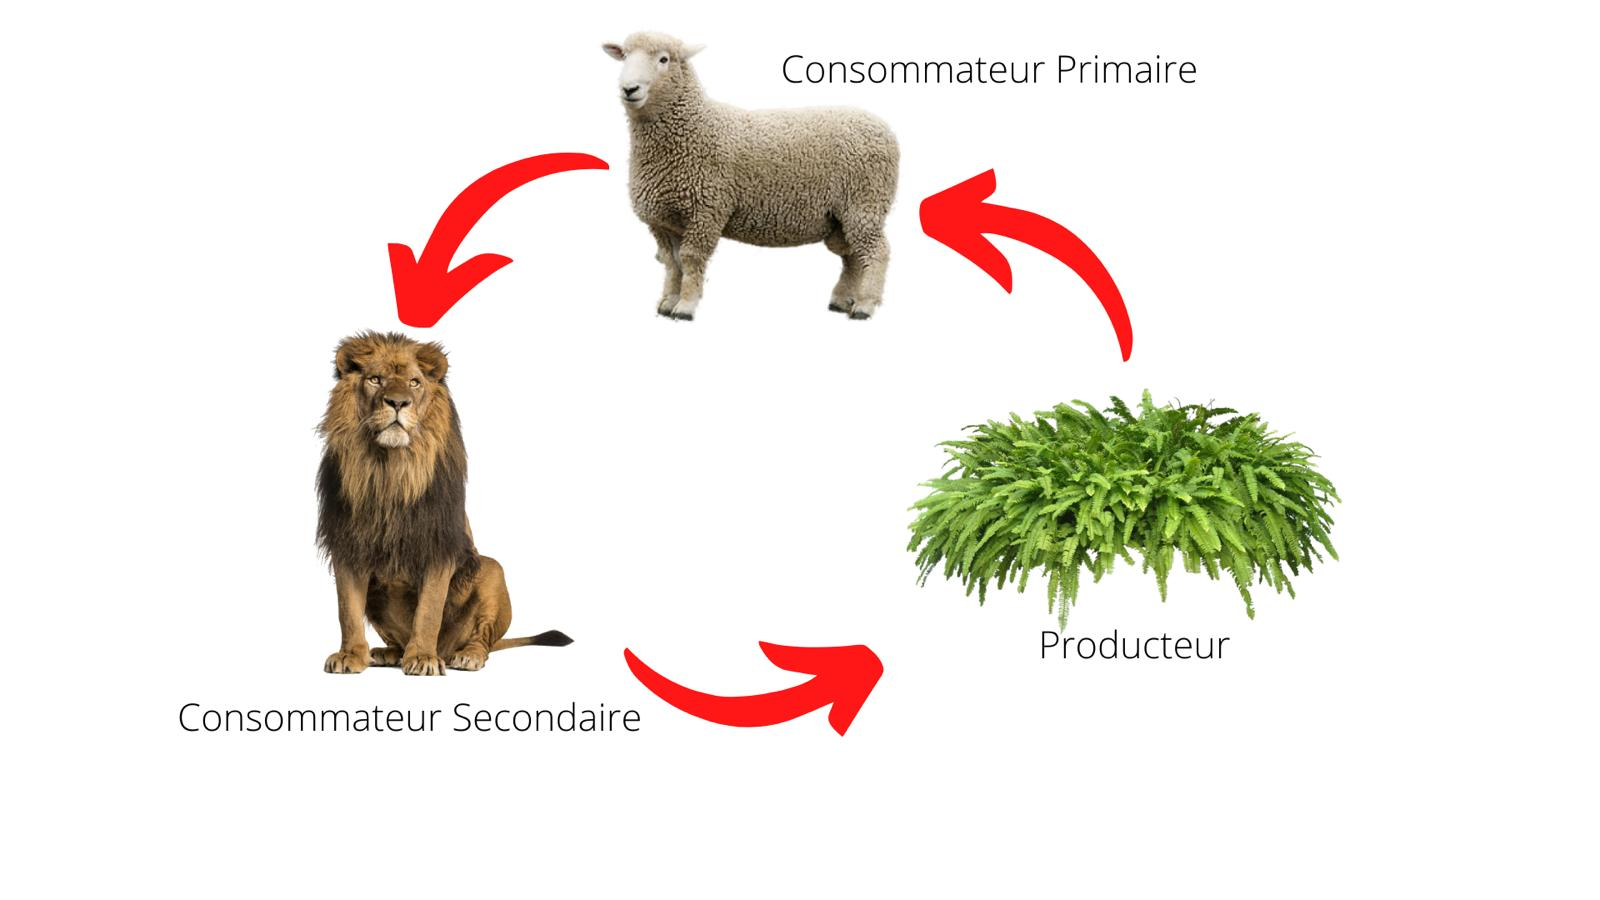
\includegraphics[width=7cm, height=5cm]{images/intro.jpeg}
    \end{figure}
\end{frame}


\section{Diagramme de classe}

\begin{frame}{Diagramme de classe}
    \begin{figure}
        \centering
        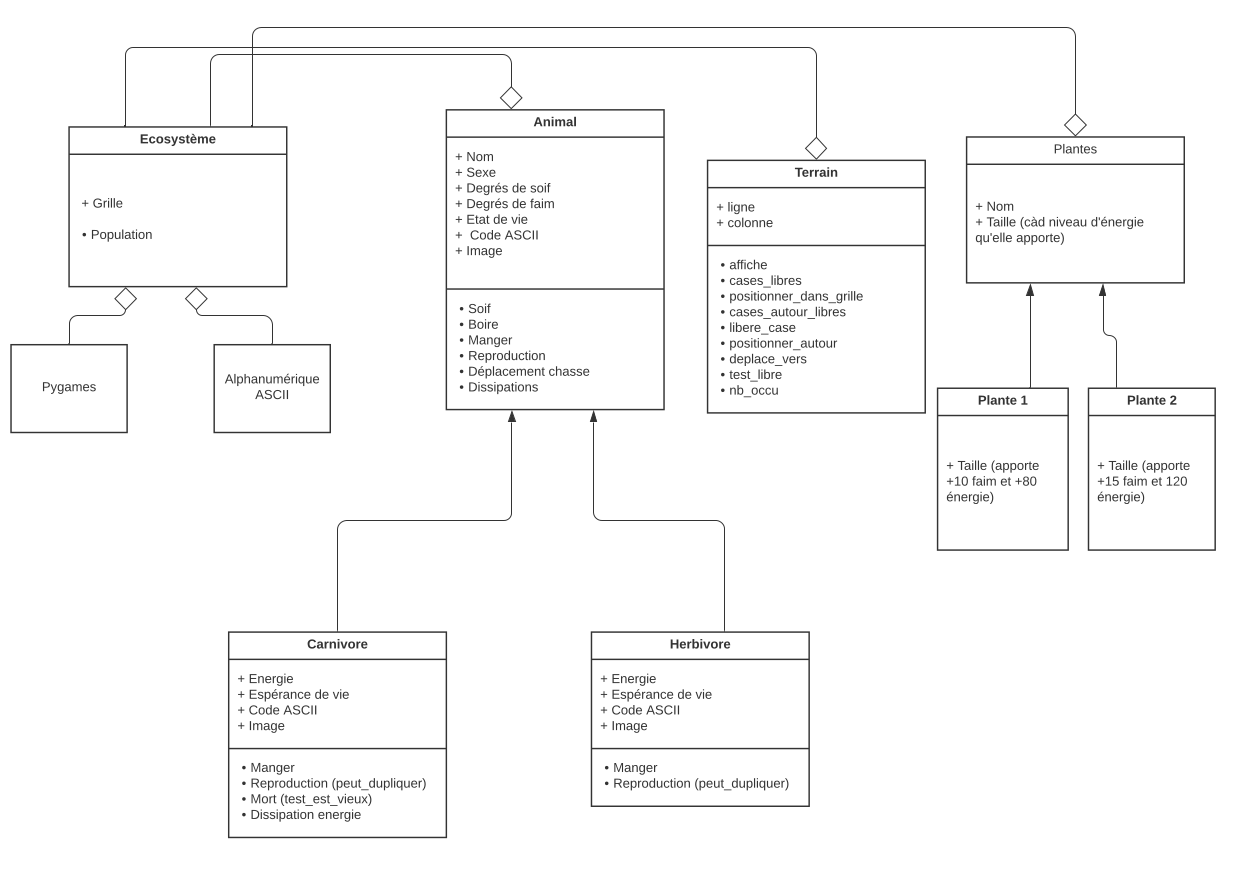
\includegraphics[width=8cm, height=6cm]{images/diagramme.png}
    \end{figure}
\end{frame}



\section{Versions du jeu}

\begin{frame}{Version du jeu}

\begin{figure}[h]
    \begin{minipage}[c]{.46\linewidth}
        \centering
        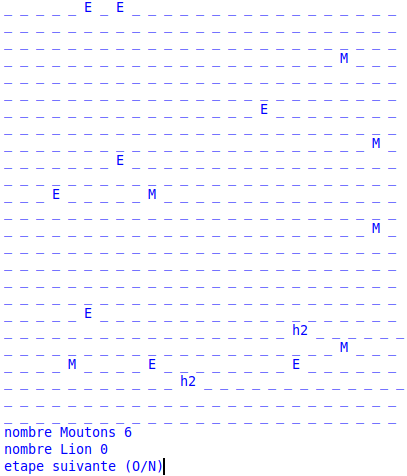
\includegraphics[width=5cm, height=4cm]{images/console.png}
    \end{minipage}
    \hfill%
    \begin{minipage}[c]{.46\linewidth}
        \centering
        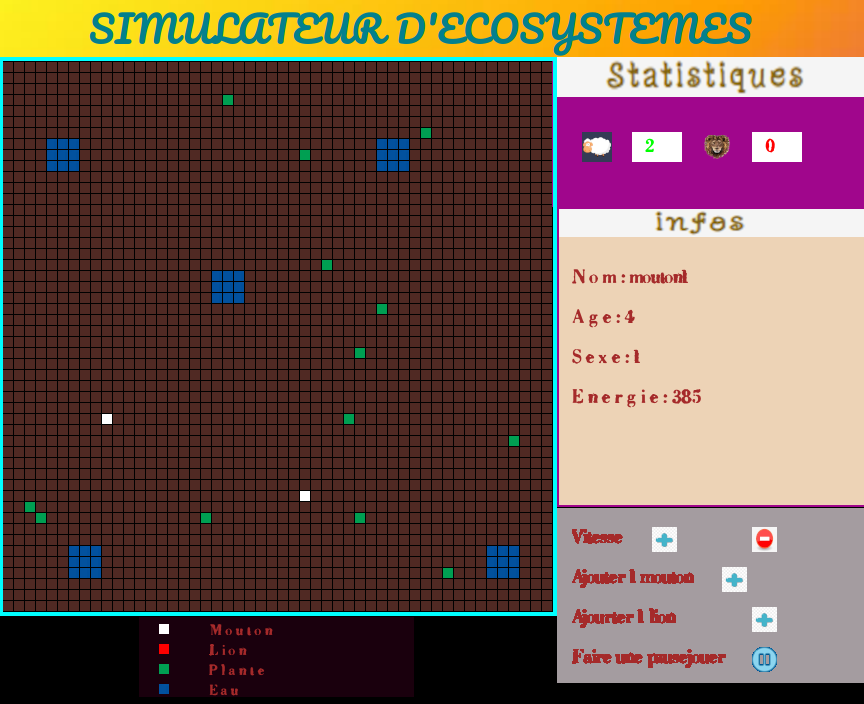
\includegraphics[width=5cm, height=4cm]{images/interface.png}
    \end{minipage}
\end{figure}
    
\end{frame}


\section{Élément techniques}

\subsection{Déplacements}
\begin{frame}{Principe déplacement }
    \hspace{0.2cm} Le simulateur se base principalement sur la fonction de déplacement d'un animal de la position (x,y) vers (a,b).\\
    \vspace{0.3cm}
    \hspace{0.2cm}Le déplacement se fait grace à une succession d'incrémentations et de decrémentation de (x,y) jusqu'a ce qu'on arrive au coordonnées (a,b).
    \begin{center}
            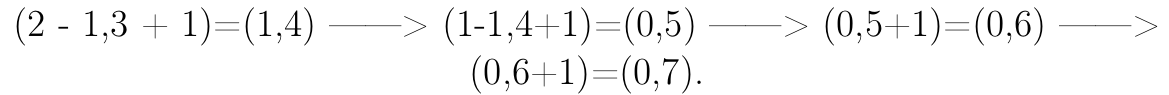
\includegraphics[keepaspectratio, scale=0.22]{images/dep.png}
        \end{center}
\end{frame}

\begin{frame}{Type de déplacements }
    Durant la simulation deux type de déplacements presque similaires s'effectuent à chaque itération : \\
    \vspace{0.3cm}
    \begin{itemize}
        \item Déplacement d'un animal pour qu’il puisse s’abreuver.
        \vspace{0.3cm}
        \item Déplacer un animal pour qu’il puisse manger.
    \end{itemize}
\end{frame}
\begin{frame}{Déplacement pour boire}
    \begin{center}
            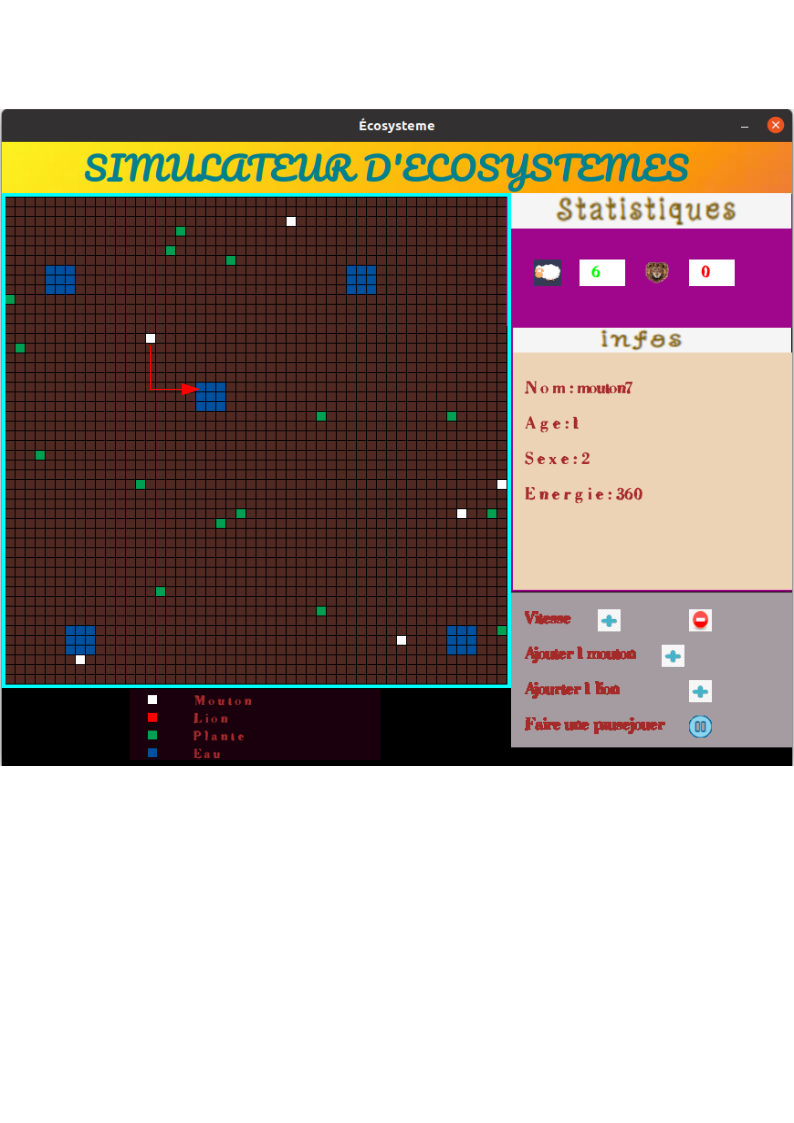
\includegraphics[keepaspectratio, scale=0.22]{images/depb.png}
    \end{center}
\end{frame}
\begin{frame}{Déplacement pour manger}
    \begin{center}
            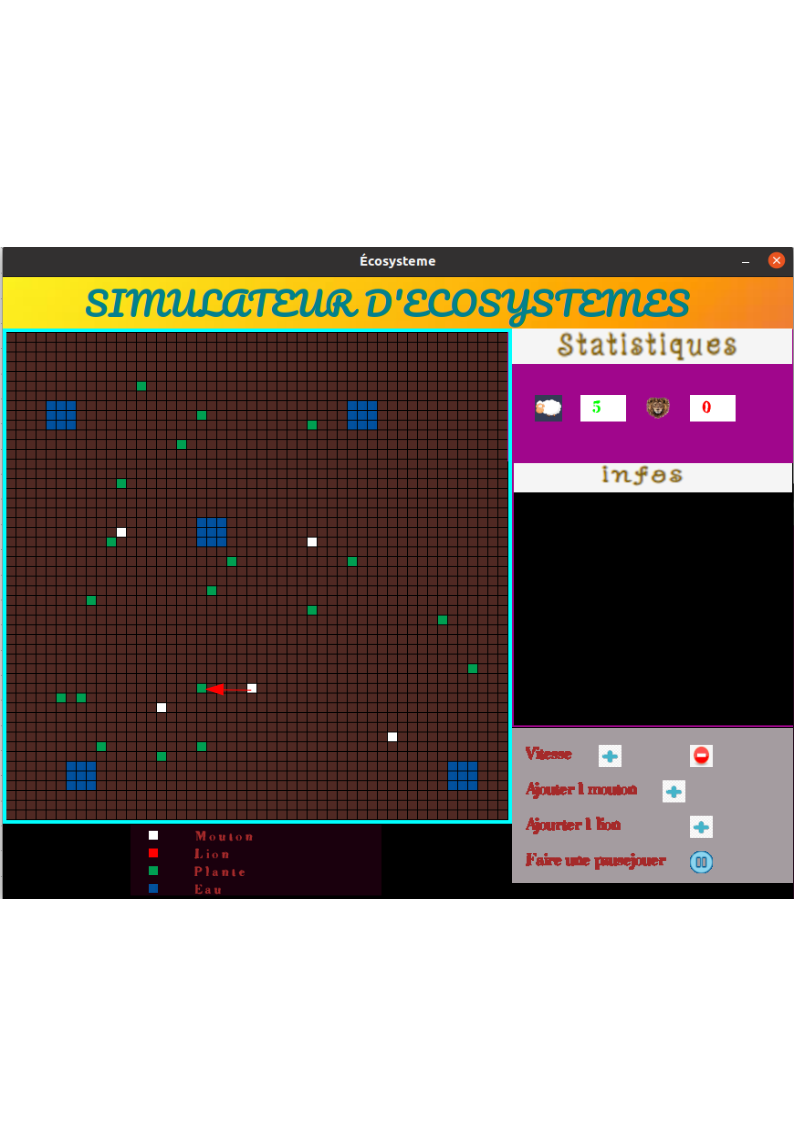
\includegraphics[keepaspectratio, scale=0.22]{images/depm.png}
    \end{center}
\end{frame}
\begin{frame}{Interaction avec l'utilisateur}
    \begin{center}
            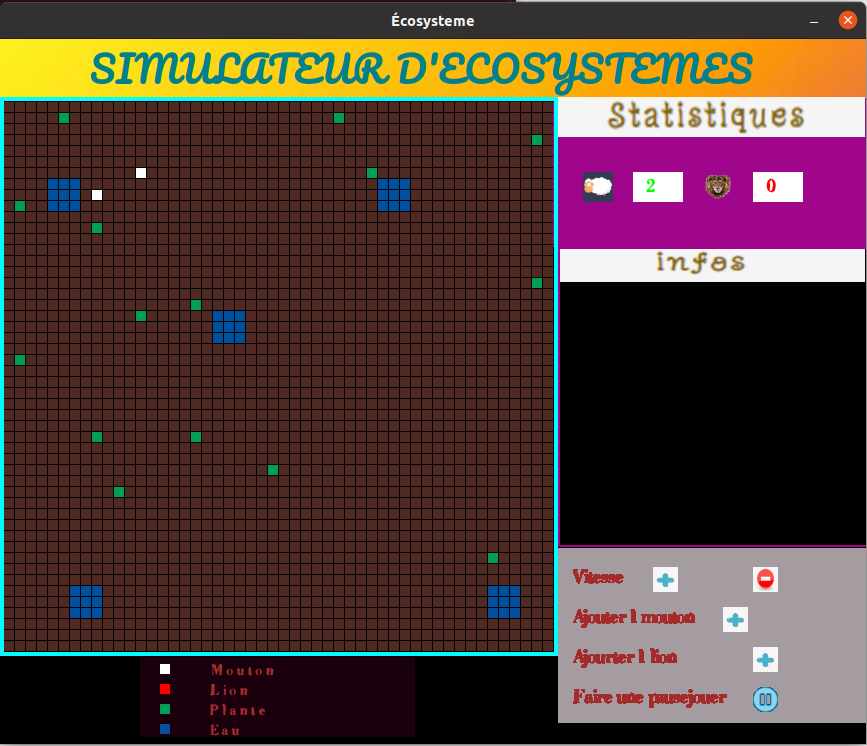
\includegraphics[keepaspectratio, scale=0.22]{images/interact.png}
    \end{center}
\end{frame}












\section{Expérimentations et équilibre}
%
\begin{frame}{Expérimentations et équilibre}
    \begin{figure}[h]
        \begin{minipage}[c]{.46\linewidth}
            \centering
            
\includegraphics[width=5cm, height=3cm]{images/experi.png}
        \end{minipage}
        \hfill%
        \begin{minipage}[c]{.46\linewidth}
            \centering
            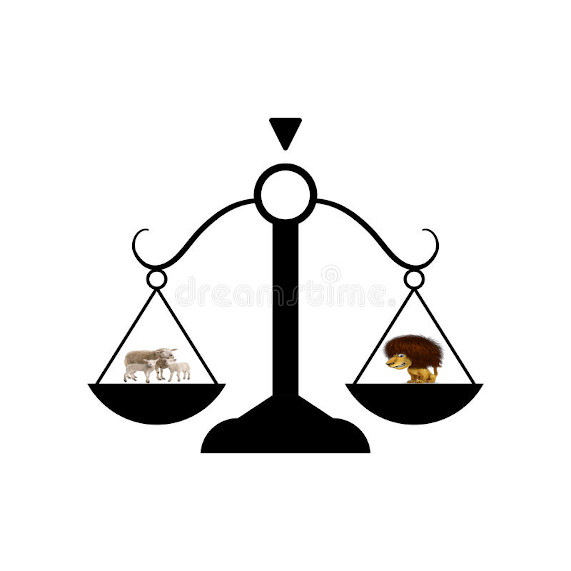
\includegraphics[width=5cm, height=5cm]{images/balance.jpg}
        \end{minipage}
    \end{figure}
\end{frame}

\subsection{Expérimentations}

\begin{frame}{Expérimentations}
    \begin{block}{Équations de Lokta-Voltera}
        \begin{equation}
             \lbrace_{\frac{dy(t)}{dt}  =  y(t)(cx(t) - d)} ^{\frac{dx(t)}{dt} = x(t)(a - by(t))}
        \end{equation}
    \end{block}
    
    Ou x(t) est l'effectif des proies, y(t) celui des prédateurs les coefficients a,b,c et d à déterminer expérimentalement :
    \begin{alertblock}{Les coefficients}
    
	\begin{itemize}
        \item \textbf{a} le coefficient d'accroissement des proies indépendemment de prédateurs:
        \item \textbf{b} le taux de mortalité des proies du aux prédateurs
        \item \textbf{c} le coefficient d'accroissement des prédateurs en fonction des proies disponibles
        \item \textbf{d} le coefficient de mort des prédateurs en l'absence des proies
	\end{itemize}
\end{alertblock}
\end{frame}

\begin{frame}
    \begin{block}{Condition d'équilibre}
        \begin{equation}
            \lbrace_{\frac{dx(t)}{dt} = 0}^{\frac{dy(t)}{dt} = 0}
        \end{equation}
    \end{block}

\end{frame}

\begin{frame}{Observations}
    \begin{figure}[h]
        \begin{minipage}[c]{.46\linewidth}
            \centering
            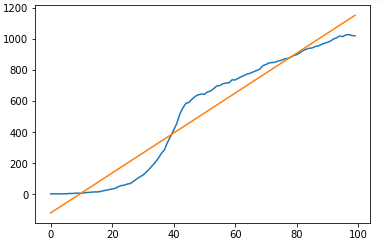
\includegraphics[width=5cm, height=2.5cm]{images/courbe1.png} 
            \caption{Détermination de \textbf{a}}
        \end{minipage}
        \hfill%
        \begin{minipage}[c]{.46\linewidth} \pause
            \centering
            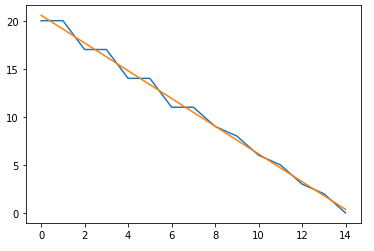
\includegraphics[width=5cm, height=2.5cm]{images/courbe2_.png} 
            \caption{Détermination de \textbf{b}}
        \end{minipage}
    \end{figure}
    
    \begin{figure}[h]
        \begin{minipage}[c]{.46\linewidth} \pause
            \centering
            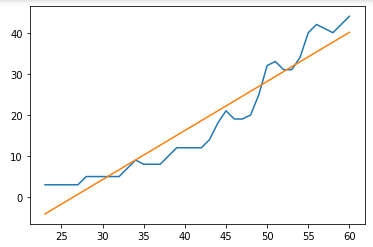
\includegraphics[width=5cm, height=2.5cm]{images/courbe3.png} 
            \caption{Détermination de \textbf{c}}
        \end{minipage}
        \hfill%
        \begin{minipage}[c]{.46\linewidth} \pause
            \centering
            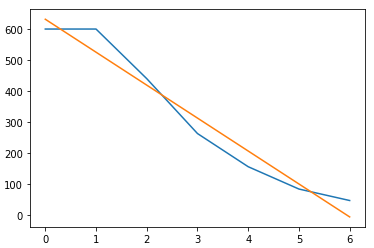
\includegraphics[width=5cm, height=2.5cm]{images/courbe2.png} 
            \caption{Détermination de \textbf{d}}
        \end{minipage}
    \end{figure}
\end{frame}


\begin{frame}{Les résultats}
    \begin{exampleblock}{Résultats}
        \begin{itemize}
            \item a = 12,57
            \item b = 1,44
            \item c = 1,31
            \item d = 17,78
	    \end{itemize}
    \end{exampleblock}
    
    Avec ces résultats, nous avons lancé une simulation et après apparition des prédateurs, on affiché les variations de populations et les résultats ne correspondaient pas à l'évolution du système.
    
    \begin{figure}[h] \pause
        \centering
        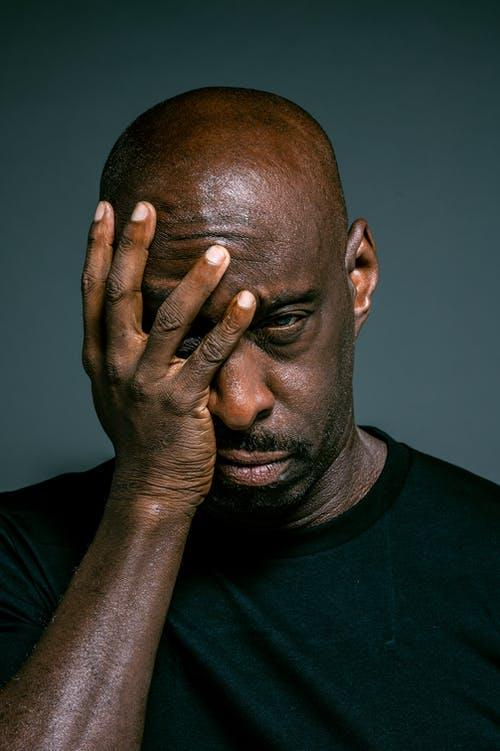
\includegraphics[width=4cm, height=2.5cm]{images/deception.jpg} 
    \end{figure}
    
\end{frame}

\begin{frame}{courbe d'évolution}
    \begin{figure}[h]
        \centering
    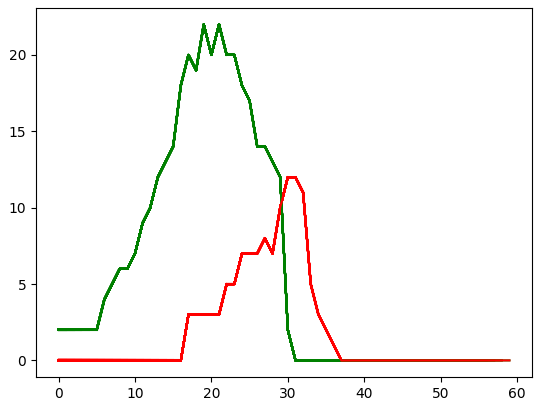
\includegraphics[width=5.5cm, height=3.5cm]{images/non_eq.png}
    \caption{Aspect de la courbe d'évolution du système}
    \end{figure}
\end{frame}

\subsection{Equilibre}

\begin{frame}{Solution pour éuilibrer le système}
        \begin{figure}[h]
        
\includegraphics[width=5.5cm, height=3.5cm]{images/idee.jpg}
        \centering
    \end{figure}
    Vu que les coefficients ne correspondaient pas, nous avons opté pour un rajout de nouvelles règles à notre système.
\end{frame}

\begin{frame}{Solution}
    \begin{figure}[h]
        \begin{minipage}[c]{.46\linewidth}
            \centering
            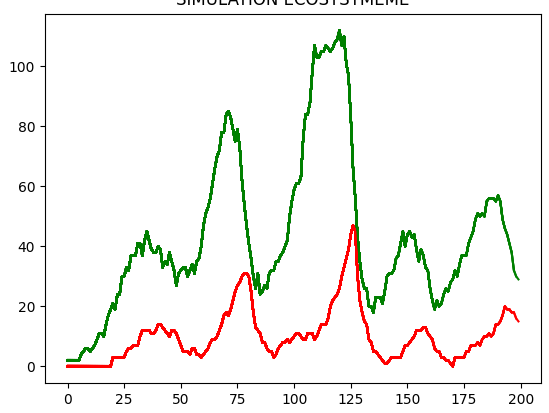
\includegraphics[width=5cm, height=2.5cm]{images/eq.png} 
        \end{minipage}
        \hfill%
        \begin{minipage}[c]{.46\linewidth} \pause
            \centering
            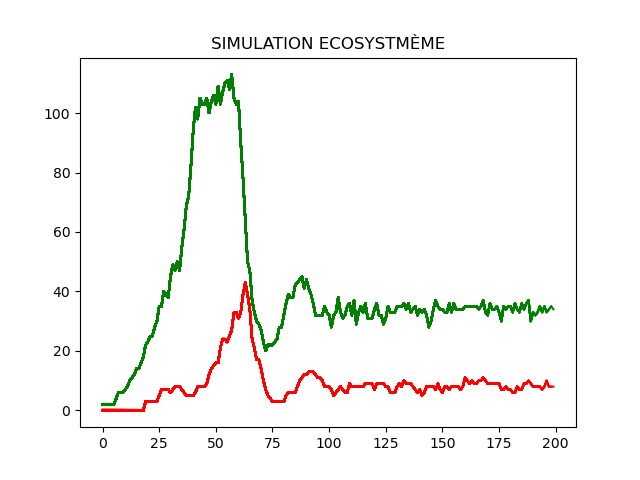
\includegraphics[width=5cm, height=2.5cm]{images/particu.png} 
        \end{minipage}
    \end{figure}
\end{frame}

\section{Conclusion}

\begin{frame}{Conclusion}
    \center CONCLUSION
\end{frame}

\end{document}